
%    \documentclass[journal,a4paper]{IEEEtran}
   \documentclass[10pt,twocolumn,twoside]{IEEEtran}

%% 88mm column width
% 18.2cms full page

   % \documentclass[draftcls,onecolumn]{IEEEtran} 
   % \topmargin       -6.0mm
   %  \oddsidemargin      0mm
   %  \evensidemargin     0mm
   %  \textheight     223.5mm
   % \textwidth      170.0mm




% If IEEEtran.cls has not been installed into the LaTeX system files,
% manually specify the path to it like:
% \documentclass[journal]{../sty/IEEEtran}





% Some very useful LaTeX packages include:
% (uncomment the ones you want to load)


% *** MISC UTILITY PACKAGES ***
%
%\usepackage{ifpdf}
% Heiko Oberdiek's ifpdf.sty is very useful if you need conditional
% compilation based on whether the output is pdf or dvi.
% usage:
% \ifpdf
%   % pdf code
% \else
%   % dvi code
% \fi
% The latest version of ifpdf.sty can be obtained from:
% http://www.ctan.org/tex-archive/macros/latex/contrib/oberdiek/
% Also, note that IEEEtran.cls V1.7 and later provides a builtin
% \ifCLASSINFOpdf conditional that works the same way.
% When switching from latex to pdflatex and vice-versa, the compiler may
% have to be run twice to clear warning/error messages.






% *** CITATION PACKAGES ***
%
\usepackage{cite}


% *** GRAPHICS RELATED PACKAGES ***
%
\ifCLASSINFOpdf
   \usepackage[pdftex]{graphicx}
  % declare the path(s) where your graphic files are
  % \graphicspath{{../pdf/}{../jpeg/}}
  % and their extensions so you won't have to specify these with
  % every instance of \includegraphics
  % \DeclareGraphicsExtensions{.pdf,.jpeg,.png}
\else
  % or other class option (dvipsone, dvipdf, if not using dvips). graphicx
  % will default to the driver specified in the system graphics.cfg if no
  % driver is specified.
  % \usepackage[dvips]{graphicx}
  % declare the path(s) where your graphic files are
  % \graphicspath{{../eps/}}
  % and their extensions so you won't have to specify these with
  % every instance of \includegraphics
  % \DeclareGraphicsExtensions{.eps}
\fi


% *** MATH PACKAGES ***
%
\usepackage[cmex10]{amsmath}
\interdisplaylinepenalty=2500

\usepackage{amssymb}




% *** ALIGNMENT PACKAGES ***
%
\usepackage{array}



%\usepackage{mdwmath}
%\usepackage{mdwtab}
% Also highly recommended is Mark Wooding's extremely powerful MDW tools,
% especially mdwmath.sty and mdwtab.sty which are used to format equations
% and tables, respectively. The MDWtools set is already installed on most
% LaTeX systems. The lastest version and documentation is available at:
% http://www.ctan.org/tex-archive/macros/latex/contrib/mdwtools/



% *** SUBFIGURE PACKAGES ***
% \usepackage[tight,footnotesize]{subfigure}

 \ifCLASSOPTIONcompsoc
  \usepackage[tight,normalsize,sf,SF]{subfigure}
\else
  \usepackage[tight,footnotesize]{subfigure}
\fi


%\usepackage[caption=false]{caption}
%\usepackage[font=footnotesize]{subfig}
% subfig.sty, also written by Steven Douglas Cochran, is the modern


% *** FLOAT PACKAGES ***
%
%\usepackage{fixltx2e}
% fixltx2e, the successor to the earlier fix2col.sty, was written by
% Frank Mittelbach and David Carlisle. This package corrects a few problems
% in the LaTeX2e kernel, the most notable of which is that in current
% LaTeX2e releases, the ordering of single and double column floats is not
% guaranteed to be preserved. Thus, an unpatched LaTeX2e can allow a
% single column figure to be placed prior to an earlier double column
% figure. The latest version and documentation can be found at:
% http://www.ctan.org/tex-archive/macros/latex/base/



\usepackage{stfloats}
% stfloats.sty was written by Sigitas Tolusis. This package gives LaTeX2e
% the ability to do double column floats at the bottom of the page as well
% as the top. (e.g., "\begin{figure*}[!b]" is not normally possible in
% LaTeX2e). It also provides a command:
%\fnbelowfloat
% to enable the placement of footnotes below bottom floats (the standard
% LaTeX2e kernel puts them above bottom floats). This is an invasive package
% which rewrites many portions of the LaTeX2e float routines. It may not work
% with other packages that modify the LaTeX2e float routines. The latest
% version and documentation can be obtained at:
% http://www.ctan.org/tex-archive/macros/latex/contrib/sttools/
% Documentation is contained in the stfloats.sty comments as well as in the
% presfull.pdf file. Do not use the stfloats baselinefloat ability as IEEE
% does not allow \baselineskip to stretch. Authors submitting work to the
% IEEE should note that IEEE rarely uses double column equations and
% that authors should try to avoid such use. Do not be tempted to use the
% cuted.sty or midfloat.sty packages (also by Sigitas Tolusis) as IEEE does
% not format its papers in such ways.


%\ifCLASSOPTIONcaptionsoff
%  \usepackage[nomarkers]{endfloat}
% \let\MYoriglatexcaption\caption
% \renewcommand{\caption}[2][\relax]{\MYoriglatexcaption[#2]{#2}}
%\fi
% endfloat.sty was written by James Darrell McCauley and Jeff Goldberg.
% This package may be useful when used in conjunction with IEEEtran.cls'
% captionsoff option. Some IEEE journals/societies require that submissions
% have lists of figures/tables at the end of the paper and that
% figures/tables without any captions are placed on a page by themselves at
% the end of the document. If needed, the draftcls IEEEtran class option or
% \CLASSINPUTbaselinestretch interface can be used to increase the line
% spacing as well. Be sure and use the nomarkers option of endfloat to
% prevent endfloat from "marking" where the figures would have been placed
% in the text. The two hack lines of code above are a slight modification of
% that suggested by in the endfloat docs (section 8.3.1) to ensure that
% the full captions always appear in the list of figures/tables - even if
% the user used the short optional argument of \caption[]{}.
% IEEE papers do not typically make use of \caption[]'s optional argument,
% so this should not be an issue. A similar trick can be used to disable
% captions of packages such as subfig.sty that lack options to turn off
% the subcaptions:
% For subfig.sty:
% \let\MYorigsubfloat\subfloat
% \renewcommand{\subfloat}[2][\relax]{\MYorigsubfloat[]{#2}}
% For subfigure.sty:
% \let\MYorigsubfigure\subfigure
% \renewcommand{\subfigure}[2][\relax]{\MYorigsubfigure[]{#2}}
% However, the above trick will not work if both optional arguments of
% the \subfloat/subfig command are used. Furthermore, there needs to be a
% description of each subfigure *somewhere* and endfloat does not add
% subfigure captions to its list of figures. Thus, the best approach is to
% avoid the use of subfigure captions (many IEEE journals avoid them anyway)
% and instead reference/explain all the subfigures within the main caption.
% The latest version of endfloat.sty and its documentation can obtained at:
% http://www.ctan.org/tex-archive/macros/latex/contrib/endfloat/
%
% The IEEEtran \ifCLASSOPTIONcaptionsoff conditional can also be used
% later in the document, say, to conditionally put the References on a 
% page by themselves. 
\usepackage{float}
 \usepackage{hyperref}
\hypersetup{colorlinks,linkcolor=black,filecolor=black,urlcolor=black,citecolor=black}




% *** PDF, URL AND HYPERLINK PACKAGES ***
%
%\usepackage{url}
% url.sty was written by Donald Arseneau. It provides better support for
% handling and breaking URLs. url.sty is already installed on most LaTeX
% systems. The latest version can be obtained at:
% http://www.ctan.org/tex-archive/macros/latex/contrib/misc/
% Read the url.sty source comments for usage information. Basically,
% \url{my_url_here}.





% *** Do not adjust lengths that control margins, column widths, etc. ***
% *** Do not use packages that alter fonts (such as pslatex).         ***
% There should be no need to do such things with IEEEtran.cls V1.6 and later.
% (Unless specifically asked to do so by the journal or conference you plan
% to submit to, of course. )


% correct bad hyphenation here
\hyphenation{op-tical net-works semi-conduc-tor}


\begin{document}
%
% paper title
% can use linebreaks \\ within to get better formatting as desired
\title{Non-Parametric Estimation of Integro-Difference Equation Based Spatio-Temporal Systems}
%
%
% author names and IEEE memberships
% note positions of commas and nonbreaking spaces ( ~ ) LaTeX will not break
% a structure at a ~ so this keeps an author's name from being broken across
% two lines.
% use \thanks{} to gain access to the first footnote area
% a separate \thanks must be used for each paragraph as LaTeX2e's \thanks
% was not built to handle multiple paragraphs
%

\author{Parham Aram, Dean R. Freestone, 
        Michael Dewar, David B. Grayden, Visakan Kadirkamanathan~\IEEEmembership{Member,~IEEE} and Kenneth Scerri  % <-this % stops a space
\thanks{P. Aram and V. Kadirkamanathan are with the Department of Automatic Control and Systems Engineering, University of Sheffield, Sheffield, S1 3JD, U.K. (e-mail:  p.aram@sheffield.ac.uk; visakan@sheffield.ac.uk).}% <-this % stops a space
\thanks{D. R. Freestone and D. B. Grayden are with the Department of Electrical and Electronic Engineering, The University of Melbourne,
Parkville, VIC, Australia (e-mail:deanrf@unimelb.edu.au; grayden@unimelb.edu.au).}
\thanks{M. Dewar is with bit.ly, New York City, USA (e-mail:md@bit.ly)}  
\thanks{K. Scerri is with the Department of Systems and Control Engineering, University of Malta, Msida, MSD, Malta (e-mail:kenneth.scerri@um.edu.mt).}}


%\thanks{Manuscript received April 19, 2005; revised January 11, 2007.}}

% note the % following the last \IEEEmembership and also \thanks - 
% these prevent an unwanted space from occurring between the last author name
% and the end of the author line. i.e., if you had this:
% 
% \author{....lastname \thanks{...} \thanks{...} }
%                     ^------------^------------^----Do not want these spaces!
%
% a space would be appended to the last name and could cause every name on that
% line to be shifted left slightly. This is one of those "LaTeX things". For
% instance, "\textbf{A} \textbf{B}" will typeset as "A B" not "AB". To get
% "AB" then you have to do: "\textbf{A}\textbf{B}"
% \thanks is no different in this regard, so shield the last } of each \thanks
% that ends a line with a % and do not let a space in before the next \thanks.
% Spaces after \IEEEmembership other than the last one are OK (and needed) as
% you are supposed to have spaces between the names. For what it is worth,
% this is a minor point as most people would not even notice if the said evil
% space somehow managed to creep in.



% The paper headers
\markboth{IEEE TRANSACTIONS ON SIGNAL PROCESSING}%
{Aram \MakeLowercase{\textit{et al.}}: A Non-Parametric Method for Integro-Difference Equation-Based Spatio-Temporal Systems}
% The only time the second header will appear is for the odd numbered pages
% after the title page when using the twoside option.
% 
% *** Note that you probably will NOT want to include the author's ***
% *** name in the headers of peer review papers.                   ***
% You can use \ifCLASSOPTIONpeerreview for conditional compilation here if
% you desire.




% If you want to put a publisher's ID mark on the page you can do it like
% this:
%\IEEEpubid{0000--0000/00\$00.00~\copyright~2007 IEEE}
% Remember, if you use this you must call \IEEEpubidadjcol in the second
% column for its text to clear the IEEEpubid mark.



% use for special paper notices
%\IEEEspecialpapernotice{(Invited Paper)}




% make the title area
\maketitle


\begin{abstract}
%\boldmath
The integro-difference equation (IDE) is an increasingly popular mathematical model of spatio-temporal processes, such as brain dynamics, weather systems, disease spread and others. Here we develop a non-parametric framework for fusing the IDE with data. The method is based on the average (over time) spatial correlations of data to estimate the spatial mixing kernel, disturbance and the noise parameters. Synthetic examples are given to demonstrate the performance of the estimation algorithm. % The proposed method can be also applied prior to the expectation maximization (EM) algorithm to provide better and efficient state and parameter estimation.
\end{abstract}
% IEEEtran.cls defaults to using nonbold math in the Abstract.
% This preserves the distinction between vectors and scalars. However,
% if the journal you are submitting to favors bold math in the abstract,
% then you can use LaTeX's standard command \boldmath at the very start
% of the abstract to achieve this. Many IEEE journals frown on math
% in the abstract anyway.

% Note that keywords are not normally used for peerreview papers.
\begin{IEEEkeywords}
dynamic spatio-temporal modelling, integro-difference equation (IDE).
\end{IEEEkeywords}






% For peer review papers, you can put extra information on the cover
% page as needed:
% \ifCLASSOPTIONpeerreview
% \begin{center} \bfseries MEDICS Category: 3-BBND \end{center}
% \fi
%
% For peerreview papers, this IEEEtran command inserts a page break and
% creates the second title. It will be ignored for other modes.
\IEEEpeerreviewmaketitle



\section{Introduction}
\IEEEPARstart{C}{omplex} spatio-temporal behavior is found in many different systems such as aquatic ecosystems \cite{Schofield2002}, meteorological forecasting \cite{Xu2005}, air pollution \cite{Romanowicz2006}, soil temperature  \cite{Bond-Lamberty2005}, chemical processes \cite{Deng2005}, disease spread \cite{Kuo2009} and real estate market \cite{Sun2005}. Spatio-temporal mathematical modeling aims to represent dynamic system behavior simultaneously across time and space. The ability to describe the spatio-temporal dynamics of such systems has a profound effect on the manner in which we deal with the natural and man-made world. For example, meteorology..... Another example such
 
%\cite{Schofield2002,Xu2005,Romanowicz2006,Bond-Lamberty2005,Deng2005,Kuo2009,Sun2005}.  %WEINAND1972  
Techniques for modeling spatio-temporal systems are generating growing interest, both in the applied and theoretical literature. This paper deals in particular with integro-difference equation (IDE) based spatio-temporal models. Other classes of models of particular interest in the wider literature include the cellular automata (CA) \cite{Wolfram1994}, coupled map lattices (CMLs) \cite{Billings2002}, lattice dynamical wavelet neural network (LDWNN) \cite{Wei2009} and spatially correlated time series \cite{Pfeifer1980,Glasbey2008,Dewar2007}, which have all been used in a system identification context. The extent of the spatial interactions in these alternate models is determined by a spatially discrete neighborhood structure.

The focus on the IDE-based models in this work is because they have received much attention in population ecology as models for the spatio-temporal spread of organisms \cite{Kot1992,Kot1996} and in the brain dynamics to model the electrophysiological measurements \cite{Deco2008,Schiff2008,Freestone2011}. The key feature of IDE models is that they combine discrete temporal dynamics with a continuous spatial representation. The dynamics of this model are governed by a spatial mixing kernel, which defines the mapping between the current spatial field and the previous spatial field. The IDE model can be applied to data sampled both regularly and irregularly in space due to the continuous representation of each spatial field. Estimating the spatial mixing kernel and the underlying spatial field is of particular interest and can be achieved by  using conventional state-space modeling \cite{Dewar2009,Scerri2009} or in a hierarchical Bayesian framework \cite{Wikle1999,Xu2005,Wikle2011}. 

\begin{figure}[ht]
	\centering
		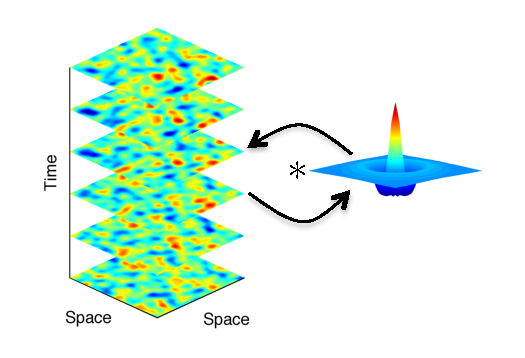
\includegraphics[scale=1]{./Graph/FieldsAndKernel_Arrows.pdf}
	\caption{caption}
	\label{fig:label}
\end{figure}

Wikle et al. \cite{Wikle2002} describe the IDE using a state-space formulation by decomposing the kernel and the field using a set of spectral basis functions. An alternative approach for the decomposition of the IDE was introduced in \cite{Dewar2009} where the resulting state and parameter space dimensions are independent of the number of observation locations. In this work a framework based on expectation maximization (EM)  algorithm \cite{Dempster1977,Gibsona2005}  was used to estimate both the field and the kernel from the observed data. A similar approach is adopted by \cite{Scerri2009} which developed a model selection procedure by considering various spatial scales at which to represent the system.  
% Therefore, increasing the resolution at which the system is observed does not necessarily increase the complexity of the system identification problem.

Here we take a different approach, using the average (over time) spatial auto-correlation and cross-correlation  of the observed field an efficient method is proposed to estimate the spatial mixing kernel, filed disturbance characteristics and the observation noise variance. This eliminates the computational load imposed by the methods in \cite{Dewar2009,Scerri2009} while they assumed that disturbance and noise characteristics were known to the estimator. Although the proposed method does not infer the underlying field from observed data, the results can be used as a prerequisite for the EM based algorithm (see \cite{Dewar2009,Xu2007}), providing better and efficient state (spatial field) and parameter estimations (spatial mixing kernel). 

The rest of this paper is set out as follows: in Section 2, the stochastic IDE model is briefly reviewed. Section 3 introduces the estimation framework and provides necessary formulations  to construct such an estimator using observed field. In Section 4, synthetic examples are given to demonstrate the performance of the developed algorithm. Finally conclusions are drawn in Section 5.


\section{Stochastic IDE Model}
The spatially homogeneous IDE is given by 
\begin{equation}
 z_{t+1}\left(\mathbf{r}\right)=\xi z_t(\mathbf{r})+T_s\int_{\Omega}k\left(\mathbf{r}-\mathbf{r}'\right)f(z_{t}\left(\mathbf{r}'\right))d\mathbf{r}'+e_{t}\left(\mathbf{r}\right),
\label{eq:ConvolutionIntegral}
\end{equation}
where $t\in \mathbb{Z}^{+} $ denotes discrete time, $T_s$ is the sampling time and $\mathbf{r} \in \Omega \subset \mathbb{R}^{n}$ are spatial locations in $n$-dimensional physical space, where $n \in \left\lbrace 1,2,3 \right\rbrace $. The dynamics of the field is included via the decay parameter $\xi$ (see \cite{Freestone2011} for more details). The continuous spatial field at time $t$ and at location $\mathbf r$ is denoted $z_t\left(\mathbf r\right)$. The model dynamics  are defined by the homogeneous time invariant spatial mixing kernel, $k\left(\mathbf{r}-\mathbf{r}'\right)$ which maps $f(z_{t})$  to the next spatial field via the integral (\ref{eq:ConvolutionIntegral}) where $f(\cdot)$ is a non-linear function. The disturbance $e_{t}(\mathbf{r})$ is a zero-mean normally distributed noise process, spatially colored but temporally independent, with covariance \cite{Rasmussen2005}
\begin{equation}
cov\left(e_{t}\left(\mathbf{r}\right),e_{t+t'}\left(\mathbf{r'}\right)\right)=\sigma_d^2\delta(t-t')\gamma(\mathbf{r}-\mathbf{r'}),
\label{eq:FieldDisturbance}
\end{equation}
where $\sigma_d$ is temporal disturbance, $\delta(\cdot)$ is the Dirac-delta function and $\gamma(\mathbf{r}-\mathbf{r'})$ is a spatially homogeneous covariance function. The mapping between the spatial field and the observations, denoted by $\mathbf{y}_t$, is modeled using the observation function that incorporates sensors with a spatial extent
\begin{equation}\label{eq:ObservationEquation}
	y_t(\mathbf{r}) = \int_{\Omega} { m\left(\mathbf{r}-\mathbf{r}'\right) z_t\left(\mathbf{r}'\right) \, d\mathbf{r}'} + \varepsilon_t(\mathbf{r}_n), 
\end{equation}
where $m\left(\mathbf{r}-\mathbf{r}'\right)$ is the observation kernel and $\varepsilon_t(\mathbf{r}_n) \sim \mathcal{N}\left(0,\boldsymbol{\Sigma}_{\varepsilon}\right)$ denotes a multivariate normal distribution with mean zero and the covariance matrix $\boldsymbol{\Sigma}_{\varepsilon} = \sigma_{\varepsilon}^2\mathbf{I}$, where $\mathbf{I}$ is the identity matrix.
% defined in this work by the Gaussian
% \begin{equation}\label{eq:observationkernel}
% 	m\left(\mathbf{r}-\mathbf{r}'\right) = \exp{\left(-\frac{(\mathbf{r}-\mathbf{r}')^\top(\mathbf{r}-\mathbf{r}')}{\sigma_m^2}\right)},
% \end{equation} 
% where $\sigma_m$ sets the observation kernel width. The superscript $\top$ denotes the transpose operator.
\section{Estimation method}\label{sec:EstimationMethod}
For the derivation of the spatial properties estimator of the field equations we assume the non-linearity is a sigmoidal function. This is common in modeling the brain dynamics to describe the firing rate of the presynaptic neurons in terms of the post-synaptic membrane potential \cite{Freeman1975} and is given by
\begin{equation}
	\label{ActivationFunction} f\left( z\left( \mathbf{r}', t \right) \right) = \frac{1}{1 + \exp \left( \varsigma \left( z_0 - z\left(\mathbf{r}',t\right) \right) \right)}. 
\end{equation}
The parameter $z_0$ describes the firing threshold of the neural populations and $\varsigma$ governs the slope of the sigmoid. The results obtained using the sigmoidal function can be easily modified to account for the linear IDE used in modeling electrophysiological data, population ecology and nowcasting. This is described in a later section in more details. To proceed we will switch to a more compact notation to define convolution and correlation operators. The spatial convolution shall be denoted as
\begin{equation}
	\int_\Omega a(\mathbf{r}-\mathbf{r}')b(\mathbf{r}')d\mathbf{r}' = (a\ast b)(\mathbf{r}),
\end{equation}
and the spatial cross-correlation shall be denoted as 
\begin{equation}
	\int_\Omega a(\mathbf{r})b(\mathbf{r}+\boldsymbol{\tau})d\mathbf{r} = (a\star b)(\boldsymbol{\tau}),
\end{equation} 
where $\boldsymbol{\tau}$ is the spatial shift.
\subsection{Estimation of spatial mixing kernel} 
Under the assumption that the sensors are not spatially band-limiting, the spectral content of the field and the spatial mixing kernel is homogeneous, the shape of the spatial mixing kernel can be inferred by studying the spatial cross-correlation between consecutive observations.  To begin the derivation we define the spatial cross-correlation between consecutive observations (in time) as  
% The spatial relationship between consecutive observations is governed by the shape of the mixing kernel. 
% The deterministic component of the spatial mapping of the current field is due to the convolution of the kernel with the previous field. Therefore, the spatial cross-correlation between consecutive observations is used to estimate the kernel's support and shape.
\begin{equation}
	R_{y_{t+1}y_t}(\boldsymbol{\tau}) = \left(y_{t+1}\star y_t\right)\left(\boldsymbol{\tau}\right).
\end{equation}
 The goal of the derivation is to make the necessary substitutions and simplifications to get an expression of the cross-correlation as a function of the mixing kernel. In the next step we substitute \eqref{eq:ObservationEquation} for $y_{t+1}(\mathbf{r})$ and expand to give
\begin{equation}
	R_{y_{t+1}y_t}\left(\boldsymbol{\tau}\right) = \left(\left(m \ast z_{t+1}\right)\star y_t\right)\left(\boldsymbol{\tau}\right) + \left(\varepsilon_{t+1} \star y_t\right)\left(\boldsymbol{\tau}\right).
\end{equation}
Next we substitute \eqref{eq:ConvolutionIntegral} for $z_{t+1}(\mathbf{r})$ giving 
\begin{align}
	R_{y_{t+1}y_t}&(\boldsymbol{\tau}) = (\left(m \ast \left(\xi z_t +  T_s g_t + e_t\right)\right) \star y_t)(\boldsymbol{\tau}) \nonumber\\
	&= \xi\left(\left(m \ast z_t\right) \star y_t \right)(\boldsymbol{\tau})+ T_s \left(\left(m\ast g_t\right)\star y_t \right)(\boldsymbol{\tau}) \nonumber\\
	&\quad+ \left(\left(m\ast e_t\right)\star y_t \right)(\boldsymbol{\tau})+ (\varepsilon_{t+1} \star y_t)(\boldsymbol{\tau}),
\end{align}
where
\begin{equation}\label{eq:averagefiringrate}
	g_t(\mathbf r)=\int_{\Omega}k\left(\mathbf{r}-\mathbf{r}'\right)f(z_{t}\left(\mathbf{r}'\right))d\mathbf{r}'.
\end{equation}
Now we take the expectation over time, so that the observation noise and process disturbance terms have minimal effect on the result, giving 
\begin{align}\label{eq:ExpectationToCancelNoise}
	\mathbf{E}[R_{y_{t+1}y_t}(\boldsymbol{\tau})] &= \mathbf{E}[\xi\left(\left(m \ast z_t\right) \star y_t \right)(\boldsymbol{\tau})] \nonumber \\
	 &\quad+ T_s \mathbf{E}[\left(\left(m\ast g_t\right)\star y_t \right)(\boldsymbol{\tau})],
\end{align}
since the disturbance and measurement noise are assumed to be independent of the observations and temporally white. Now by substituting $y_t - \varepsilon_t$   in for $m\ast z_t$ from \eqref{eq:ObservationEquation} the first term of above equation can be written as
\begin{align}
	\mathbf{E}[\xi&\left(\left(m \ast z_t \right) \star y_t \right)(\boldsymbol{\tau})] = \mathbf{E}\left[\xi\left(\left(y_t-\varepsilon_t\right) \star y_t \right)(\boldsymbol{\tau})\right] \nonumber \\
	&= \xi \mathbf{E}\left[ (y_t \star y_t)(\boldsymbol{\tau}) - \left(\varepsilon_t\star y_t \right)(\boldsymbol{\tau})\right] \nonumber \\
	&= \xi\mathbf{E}[ R_{y_ty_t}(\boldsymbol{\tau})  - \left(\varepsilon_t \star (m\ast z_t + \varepsilon_t)\right) (\boldsymbol{\tau})] \nonumber \\
	&=\xi\mathbf{E}[ R_{y_ty_t}(\boldsymbol{\tau}) -\left(\varepsilon_t\star (m\ast z_t)\right)(\boldsymbol{\tau}) - (\varepsilon_t\star\varepsilon_t)(\boldsymbol{\tau})] \nonumber\\ 
	&= \xi\left(\mathbf{E}[ R_{y_ty_t}(\boldsymbol{\tau})] - \sigma_{\varepsilon}^2 \delta(\boldsymbol{\tau})\right). \label{eq:FirstTermReduced}
\end{align}
Next we simplify second term in equation \eqref{eq:ExpectationToCancelNoise} to get an expression involving the spatial mixing kernel. By substituting equation \eqref{eq:averagefiringrate} for $g_t$ we can write
\begin{equation}\label{eq:before_linearization}
	T_s((m \ast g_t) \star y_t)(\boldsymbol\tau) = T_s((k \ast m\ast f(z_t)) \star y_t)(\boldsymbol\tau).
\end{equation}   
The remainder of the derivation is focused on isolating the spatial mixing kernel. To show how this is done, the activation function is simplified by linearizing about the threshold, $z_0$ using a first order Taylor series expansion giving
\begin{align}
	\hat{f}(z_t\left(\mathbf{r}\right)) &=\frac{2 + \varsigma(z_t\left(\mathbf{r}\right) - z_0)}{4}. 
\end{align}	
Substituting the linearized activation function back into equation~\eqref{eq:before_linearization} we get
\begin{align}	
	T_s((m \ast g_t) \star y_t)(\boldsymbol\tau) \approx \frac{T_s}{4}((k\ast (c_1 + \varsigma m \ast z_t)) \star y_t)(\boldsymbol\tau), 
\end{align}
where
\begin{equation}
	c_1 = m\ast (2 - \varsigma z_0),
\end{equation}
is a constant. Now by substituting $y_t - \varepsilon_t$ in for $m\ast v_t$ we can write
\begin{align}
	T_s((m \ast g_t) \star y_t)(\boldsymbol\tau) &\approx \frac{T_s}{4}((k\ast (c_1 + \varsigma (y_t - \varepsilon_t))) \star y_t) (\boldsymbol\tau)
\end{align}
To isolate the kernel, the order of the convolution and cross-correlation is reversed by recognizing that a property $(a \ast b)(\boldsymbol\tau) \star c(\boldsymbol\tau) = a(-\boldsymbol\tau)\ast(b \star c)(\boldsymbol\tau)$ (see Appendix~\ref{ap:CorrelationAnalysis}). Therefore,
\begin{align}
	T_s((m \ast g_t) \star y_t)(\boldsymbol\tau) &\approx \frac{T_s}{4} k(-\boldsymbol\tau) \ast ((c_1 + \varsigma (y_t - \varepsilon_t)) \star y_t)(\boldsymbol\tau) \nonumber\\
	= \frac{T_s}{4}k(-\boldsymbol\tau) & \ast (( c_t + \varsigma (y_t - \varepsilon_t)) \star y_t) (\boldsymbol\tau),
\end{align}
where
\begin{equation}
	c_t = (c_1\star y_t)(\boldsymbol\tau).
\end{equation}  
Now using the identity established to get equation~\eqref{eq:FirstTermReduced} we have
\begin{align}\label{eq:second_term_reduced}
	T_s\mathbf{E}&\left[((m \ast g_t) \star y_t)(\boldsymbol\tau)\right] \approx \nonumber \\
	&\frac{T_s}{4} k(-\boldsymbol\tau) \ast (\mathbf{E}\left[c_t\right] + \varsigma (\mathbf{E}\left[R_{y_ty_t}(\boldsymbol\tau)\right] - \sigma_{\varepsilon}^2 \delta(\boldsymbol\tau)))
\end{align}
Now substituting back to equation~\eqref{eq:second_term_reduced} into equation~\eqref{eq:ExpectationToCancelNoise}  we get
\begin{align}\label{eq:SimplifiedXcorr}
	\mathbf{E}&[R_{y_{t+1}y_t}(\boldsymbol{\tau})] \approx \xi\left(\mathbf{E}[ R_{y_ty_t}(\boldsymbol{\tau})] - \sigma_{\varepsilon}^2 \delta(\boldsymbol{\tau})\right) \nonumber \\
	&\quad+ \frac{T_s}{4} k(-\boldsymbol\tau) \ast (\mathbf{E}\left[c_t\right] + \varsigma (\mathbf{E}\left[R_{y_ty_t}(\boldsymbol\tau)\right] - \sigma_{\varepsilon}^2 \delta(\boldsymbol\tau))).
\end{align}
Rearranging equation~\eqref{eq:SimplifiedXcorr} we get
\begin{align} \label{eq:Tobesolvedforthekernel}
	k(-\boldsymbol\tau) & \ast (\mathbf{E}\left[c_t\right] + \varsigma (\mathbf{E}\left[R_{y_ty_t}(\boldsymbol\tau)\right] - \sigma_{\varepsilon}^2 \delta(\boldsymbol\tau))) \approx  \nonumber \\
	& \frac{4}{T_s}(\mathbf{E}[R_{y_{t+1}y_t}(\boldsymbol{\tau})] - \xi\left(\mathbf{E}[ R_{y_ty_t}(\boldsymbol{\tau})] - \sigma_{\varepsilon}^2 \delta(\boldsymbol{\tau})\right)).
\end{align}
The solution of the above equation for the mixing kernel is a deconvolution. Using the convolution theorem \eqref{eq:Tobesolvedforthekernel} can be solved for the kernel in the frequency domain giving,
\begin{align}
	\mathcal{F}&\{k(-\boldsymbol\tau)\} \approx  \nonumber \\
	&= \frac{4}{T_s} \frac{\mathcal{F}\{\mathbf{E}[R_{y_{t+1}y_t}(\boldsymbol{\tau})]\} - \xi\left(\mathcal{F}\{\mathbf{E}[ R_{y_ty_t}(\boldsymbol{\tau})]\} - \sigma_{\varepsilon}^2 \right)} {\mathbf{E}\left[c_t\right]\delta(\boldsymbol{\nu}) + \varsigma (\mathcal{F}\{\mathbf{E}\left[R_{y_ty_t}(\boldsymbol\tau)\right]\} - \sigma_{\varepsilon}^2 )},  \label{eq:Fourier_TF_of_Kernel}
\end{align} 
where $\boldsymbol\nu$ is the spatial frequency. Finally an expression for the kernel is obtained by taking the inverse Fourier transform giving 
\begin{align}\label{eq:EM-Fourier_TF_of_Kernel}   
	k&(\boldsymbol\tau) = \nonumber \\
	&\frac{4}{T_s}\mathcal{F}^{-1}\overline{\left\{ \frac{\mathcal{F}\{\mathbf{E}[R_{y_{t+1}y_t}(\boldsymbol{\tau})]\} - \xi\left(\mathcal{F}\{\mathbf{E}[ R_{y_ty_t}(\boldsymbol{\tau})]\} - \sigma_{\varepsilon}^2 \right)} {\mathbf{E}\left[c_t\right]\delta(\boldsymbol{\nu}) + \varsigma (\mathcal{F}\{\mathbf{E}\left[R_{y_ty_t}(\boldsymbol\tau)\right]\} - \sigma_{\varepsilon}^2 )} \right\}},
\end{align}
 where over-bar denotes the complex conjugate operator. As the mixing kernel is a real function, the complex conjugate operator essentially reflects the kernel through the origin in the spatial domain \cite{Bracewell2000}. In the case of isotropic kernel, the complex conjugate operator can be dropped. 

From \eqref{eq:EM-Fourier_TF_of_Kernel} we see that an error in our guess for $\xi$ will result in a shift of the estimated kernel amplitude. An incorrect estimate of $c_t$ will result in a DC scaling in the kernel estimate and an error in the initial guess of  the observation noise variance will result in a distortion in the shape of the kernel, however if the signal-to-noise ratio is high such a distortion becomes insignificant.
By the Wiener-Khintchine theorem (WKT) the second terms in nominator and denominator of \eqref{eq:EM-Fourier_TF_of_Kernel} are equivalent to the power spectral density (PSD) which is non-negative and a real quantity \cite{Ricker2003}. The WKT allows to establish the bounds on the initial guess of $\sigma_{\varepsilon}^2$
% The WKT states that the power spectral density of the wide sense stationary process is the Fourier transform of its auto-correlation function .
\begin{equation}\label{eq:BoundOnObsVariance}   
  \min\mathcal{F}\{(\mathbf{E}\left[R_{y_ty_t}(\boldsymbol\tau)\right]\}\ge\sigma_{\varepsilon}^2\ge0. 
\end{equation}
\subsection{Estimation of disturbance covariance function}
The field disturbance at each spatial location and at a given time is correlated with other spatial locations through the disturbance covariance
function, suggesting the auto-correlation of the observed field at each time instant may provide useful information about the field disturbance characteristics.
The observation auto-correlation at time $t+1$ can be expressed as
\begin{equation}\label{eq:EM-ObservationEquationAutocorrelation}
	R_{y_{t+1}y_{t+1}}(\boldsymbol{\tau})=(y_{t+1} \star y_{t+1})(\boldsymbol\tau).
\end{equation}
 After substituting for $y_{t+1}$ from \eqref{eq:ObservationEquation} and using \eqref{eq:ConvolutionIntegral}   for $z_{t+1}$,  \eqref{eq:EM-ObservationEquationAutocorrelation} is expanded to give 
\begin{align}\label{eq:EM-expanded_auto_corr}  
	R_{y_{t+1}y_{t+1}} & (\boldsymbol{\tau}) = \\ \nonumber 
	\left( \left(\xi( m\ast z_{t}) \right.\right.&+\left.\left. T_s(m\ast g_{t}) + ( m \ast e_{t})+\varepsilon_{t+1} \right) \star y_{t+1} \right) (\boldsymbol{\tau})
\end{align}
Now expanding we get
\begin{align}\label{eq:expanded_auto_corr}
	R_{y_{t+1}y_{t+1}}&(\boldsymbol{\tau}) = \xi((m \ast z_{t}) \star y_{t+1})(\boldsymbol{\tau})+T_s((m\ast g_{t})\star y_{t+1})(\boldsymbol{\tau}) \nonumber \\
	&\quad+((m\ast e_{t})\star  y_{t+1})(\boldsymbol{\tau})+(\varepsilon_{t+1} \star y_{t+1})(\boldsymbol{\tau}).
\end{align}
By using similar arguments that were used in the derivation for the mixing kernel, the auto-correlation can be simplified by recognizing that
\begin{align}\label{eq:EM-Autoterm1} 
  \mathbf{E}[\xi((m\ast z_{t})\star y_{t+1})(\boldsymbol{\tau})]&=\xi \mathbf{E}[ R_{y_ty_{t+1}}(\boldsymbol{\tau})],
\end{align}
\begin{align}\label{eq:EM-Autoterm2}
 (\varepsilon_{t+1}\star y_{t+1})(\boldsymbol\tau)&=\sigma_{\varepsilon}^2\delta(\boldsymbol{\tau}),
\end{align} 
and
\begin{align}\label{eq:EM-Autoterm3} 
	T_s\mathbf{E}[((m\ast g_t) &\star y_{t+1})(\boldsymbol\tau)] \nonumber \\ 
	&\approx \frac{T_s}{4}\mathbf{E}[((m \ast k \ast (2 + \varsigma z_t - \varsigma z_0))\star y_{t+1})(\boldsymbol\tau)] \nonumber \\
	&= \frac{T_s}{4} w(-\boldsymbol\tau) \ast (\mathbf{E}\left[c_t\right] + \varsigma \mathbf{E}\left[R_{y_ty_{t+1}}(\boldsymbol\tau)\right] ).
\end{align}
Substituting \eqref{eq:EM-Autoterm1}, \eqref{eq:EM-Autoterm2} and ~\eqref{eq:EM-Autoterm3} back into \eqref{eq:expanded_auto_corr} and taking the expectation over time  gives
\begin{align}\label{eq:Auto&CrossNoisy}
	\mathbf{E}&[R_{y_{t+1}y_{t+1}}(\boldsymbol{\tau})] = \xi \mathbf{E}[R_{y_ty_{t+1}}(\boldsymbol{\tau})] \nonumber \\
	&\quad+  \frac{T_s}{4} k(-\boldsymbol\tau) \ast (\mathbf{E}\left[c_t\right] + \varsigma \mathbf{E}\left[R_{y_ty_{t+1}}(\boldsymbol\tau)\right] ) \nonumber \\
	&\quad+\mathbf{E}[((m\ast e_t)\star y_{t+1})(\boldsymbol\tau)]+\sigma_{\epsilon}^2\delta(\boldsymbol{\tau}).
\end{align}
The third term in \eqref{eq:Auto&CrossNoisy} can be simplified as 
\begin{align}\label{eq:term3Noisy}
\mathbf{E}&[((m\ast e_t)\star y_{t+1})(\boldsymbol\tau)] \nonumber \\
  &=\mathbf{E}[((m\ast e_t)\star (m\ast z_{t+1}+\varepsilon_{t+1})) (\boldsymbol\tau)] \nonumber \\
	&= \mathbf{E}[(\left(m \ast e_t\right) \star (m \ast [\xi z_t+ T_s g_t + e_t]+\varepsilon_{t+1}))(\boldsymbol\tau)] \nonumber \\
	&=\mathbf{E}[\left(m \ast e_t\right)\star\left(m \ast e_t\right)(\boldsymbol\tau)]
\end{align} 
This holds as the disturbance, $e_t$, is not correlated with the field, $z_t$, and the observation noise, $\varepsilon_{t+1}$. A property of cross-correlation and convolution is $(a \ast b)(\boldsymbol\tau) \star (a \ast b)(\boldsymbol\tau)=(a \star a)(\boldsymbol\tau)\ast(b \star b)(\boldsymbol\tau)$ (see Appendix~\ref{ap:CorrelationAnalysis}). By using this relationship and the isotropy property of the observation kernel \eqref{eq:term3Noisy} can be written as
\begin{align}\label{eq:EM-Autoterm4}
\mathbf{E}[(\left(m \ast e_t\right)\star\left(m \ast e_t\right))(\boldsymbol\tau)]&=\mathbf{E}[(\left(m \star m\right)\ast\left(e_t \star e_t\right))(\boldsymbol\tau)] \nonumber \\
&=(m\ast m \ast \gamma)(\boldsymbol\tau).
\end{align}
Substituting this back into \eqref{eq:Auto&CrossNoisy}  gives
\begin{align}
	\mathbf{E}&[R_{y_{t+1}y_{t+1}}(\boldsymbol{\tau})] = \xi \mathbf{E}[R_{y_ty_{t+1}}(\boldsymbol{\tau})] \nonumber \\
	&\quad+  \frac{T_s}{4} k(-\boldsymbol\tau) \ast (\mathbf{E}\left[c_t\right] + \varsigma \mathbf{E}\left[R_{y_ty_{t+1}}(\boldsymbol\tau)\right] ) \nonumber \\
	&\quad+(m\ast m \ast \gamma)(\boldsymbol\tau)+\sigma_{\varepsilon}^2\delta(\boldsymbol{\tau}).
\end{align}
To solve for the disturbance covariance function, once again the convolution theorem is used. Taking the Fourier transform and rearranging gives
\begin{align}
	\mathcal{F}&\{(m\ast m \ast \gamma)(\boldsymbol\tau)\} = \mathcal{F}\{\mathbf{E}[R_{y_{t+1}y_{t+1}}(\boldsymbol{\tau})]\}-\sigma_{\varepsilon}^2 \nonumber \\ 
	&\quad-\xi \mathcal{F}\{\mathbf{E}[R_{y_ty_{t+1}}(\boldsymbol{\tau})]\} \nonumber \\
	&\quad - \frac{T_s}{4} \mathcal{F}\{k(-\boldsymbol\tau)\}\mathcal{F}\left\{\mathbf{E}\left[c_t\right] + \varsigma \mathbf{E}\left[R_{y_ty_{t+1}}(\boldsymbol\tau)\right] \right\},
\end{align}
 rearranging and taking the inverse Fourier transform yields the final result 
 \begin{align}\label{eq:EM-MMGFourier2}   
	\gamma&(\boldsymbol\tau) =\mathcal{F}^{-1}\left\lbrace\frac{1}{\tilde{m}(\boldsymbol\tau)}\Bigg[\left[ \mathcal{F}\{\mathbf{E}[R_{y_{t+1}y_{t+1}}(\boldsymbol{\tau})]\}-\sigma_{\varepsilon}^2  \nonumber \right. \right. \\ 
	&\quad-\xi \mathcal{F}\{\mathbf{E}[R_{y_ty_{t+1}}(\boldsymbol{\tau})]\} \nonumber \\
	&\left.\quad - \frac{T_s}{4} \mathcal{F}\{k(-\boldsymbol\tau)\}\mathcal{F}\left\{\mathbf{E}\left[c_t\right] + \varsigma \mathbf{E}\left[R_{y_ty_{t+1}}(\boldsymbol\tau)\right] \right\}\Bigg]\right\rbrace,
\end{align}
where
\begin{equation}
 \tilde{m}(\boldsymbol\tau)=\mathcal{F}\{m(\boldsymbol\tau)\}\mathcal{F}\{m(\boldsymbol\tau)\}.
\end{equation}
% from \eqref{eq:EM=mmgamma},  when considering a sensor with a spatial extent equation \eqref{eq:EM-MMGFourier2} should be used
Using the result obtained for the kernel from  \eqref{eq:Fourier_TF_of_Kernel}  the equation for covariance function can be solved. From \eqref{eq:EM-MMGFourier2}, to calculate the exact shape of the disturbance covariance function, in addition to the parameters affecting the spatial mixing kernel the observation noise variance and the sensor kernel support are required. Similarly an estimate  of $\sigma_{\varepsilon}^2$ can be found using \eqref{eq:BoundOnObsVariance}. If $m(\cdot)$ is a point sensor then the shape of $\gamma(\cdot)$ can be calculated directly, when considering a sensor with a spatial extent, dividing by $\tilde{m}(\boldsymbol\tau)$ in \eqref{eq:EM-MMGFourier2} is then required. 
Note using uniform observation samples in \eqref{eq:EM-Fourier_TF_of_Kernel}  and \eqref{eq:EM-MMGFourier2} provide an approximate solution to the estimated  mixing kernel and disturbance covariance function. 
\begin {table}[t]
\begin{center}
	{\tiny\begin{tabular}{llll}
	\hline \hline
	& Symbol & Quantity & Units\\ 
	\hline 
	& Domain and indices&& \\
	& $\Omega$ &Spatial domain& n.a. \\ 
	& $\mathbb{Z}^{+}$ &Non-negative integers& n.a. \\ 
	& $\mathbf{r}$ &Spatial location& arbitrary unit\\ 
	& $t$ &Time & s \\  
 	& $\boldsymbol{\nu}$ &Spatial frequency& arbitrary unit\\  
	& $\mathbf I$ & Identity matrix & n.a. \\
	& Model&& \\ 
	& $\mathbf{y}_t$ & Observation & Arbitrary unit \\
	& $z_t(\mathbf{r})$ & Spatial field & Arbitrary unit \\ 
	& $f_t(\mathbf{r})$ & Sigmoidal function & spike~s$^{-1}$ \\ 
	& $g_t(\mathbf{r})$ & Weighted sigmoidal function & spike~s$^{-1}$ \\
 	& $e_t(\mathbf{r})$ & Field disturbance, with covariance function $\gamma(\mathbf{r}-\mathbf{r'})$  & spike~s$^{-1}$ \\
 
	
	\hline \hline
	\end{tabular}}
 \caption {{\bf Cardinal B-Splines at the knot sequence}.} 
 \label{table:MRA-BsplineatIntegerPoints}
 \end{center}
 \end {table}
\section{Simulation}   
\begin{figure}[ht]
	\centering
		\subfigure[]{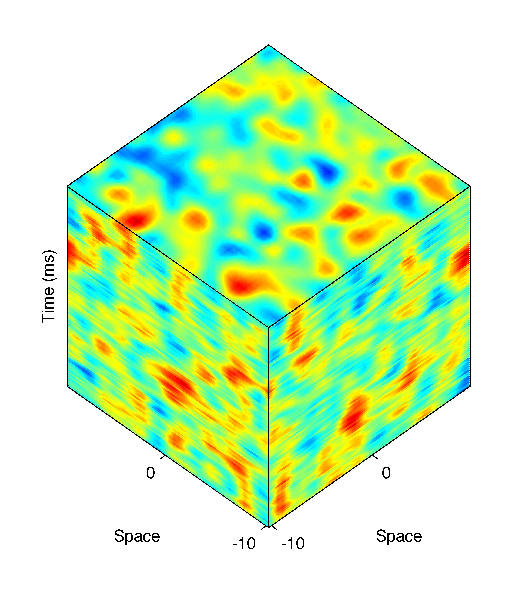
\includegraphics[scale=1]{./Graph/100Fields.pdf}}
		\subfigure[]{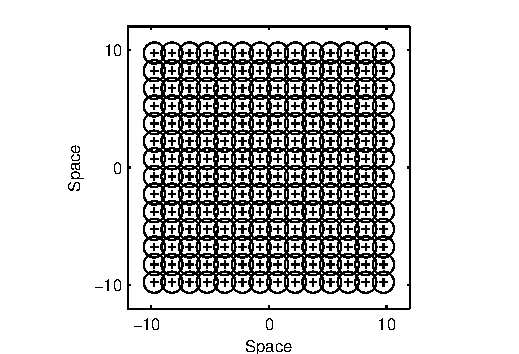
\includegraphics[scale=1]{./Graph/SensorArrangement.pdf}}
	\caption{caption}
	\label{fig:label}
\end{figure}

This section demonstrates the performance of the proposed estimation scheme. Two examples are shown where different spatial mixing kernels (isotropic and anisotropic) were adopted. These kernels are defined as a sum of Gaussian basis functions in the form of
\begin{align}\label{eq:sumofGaussians}
 k\left(\mathbf{r}-\mathbf{r}'\right)=\sum_{i=0}^{n_{\theta}}\theta_i\psi_i\left(\mathbf{r}-\mathbf{r}'\right), 
 \end{align}
where $\theta_i$ is the weight and
\begin{equation}\label{eq:Kernelbasis}
	\psi_i=\exp{\left(-\frac{(\mathbf{r}-\mathbf{r}'-\boldsymbol\mu_i)^\top(\mathbf{r}-\mathbf{r}'-\boldsymbol\mu_i)}{\sigma_i^2}\right)}.
\end{equation}
 In each example data was generated using \eqref{eq:ConvolutionIntegral} and \eqref{eq:ObservationEquation} over the spatial region $\mathcal{S}=[-10,10]^2 $, assuming periodic boundary condition (PBC), and sampled over $t=\left\lbrace1 \cdots 10000  \right\rbrace $ at 196 regularly spaced locations, with the sensor kernel defined by \eqref{eq:observationkernel} where $\sigma_m^2=0.81$. The observation noise variance $\sigma_{\varepsilon}^2$ is set to $0.1$. The field disturbance covariance function, $\gamma(\cdot)$ is modeled by a Gaussian with the width $\sigma_{\gamma}^2=1.3$ and $\sigma_d^2=0.1$. First 1000 samples discarded allowing the model's initial transients to die out. Examples of the simulated fields for each experiment at the final time instant are shown in \figurename{\ref{fig:field}}, showing stable dynamics. 

In the experiments first $\sigma_{\varepsilon}^2$ is estimated using the minimum defined by inequality \eqref{eq:BoundOnObsVariance}. The estimated variance is then used in the formulations given by \eqref{eq:EM-KernelSolution} and \eqref{eq:EM-MMGFourier2} to estimate the kernel and the disturbance function, i.e. $\sigma_d^2\gamma(\mathbf{r}-\mathbf{r'})$.
% \begin{figure}[!h] 
%  \centering
%  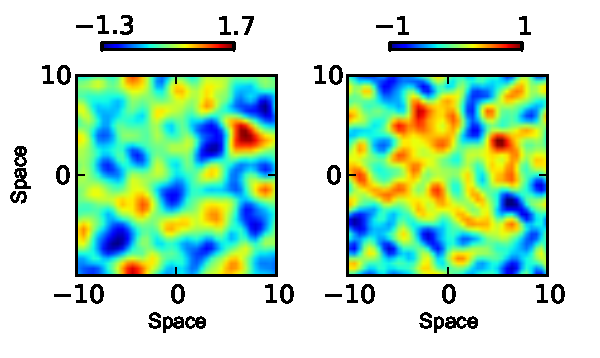
\includegraphics[width=0.5\textwidth]{./Graph/FieldSnapshot.pdf}
%  \caption{Snapshots of the underlying fields using different spatial mixing kernels; left and right panels are the generated periodic fields using isotropic (Mexican-hat shape) and anisotropic spatial mixing kernels at the final time step.}
%  \label{fig:field}
%  \end{figure}    
\subsection{Example I: isotropic mixing kernel}
 Consider the following homogeneous mixing kernel with $n_\theta=2$, $\boldsymbol\mu_0=\boldsymbol\mu_1=\mathbf 0$, $\sigma_0^2=3.24$, $\sigma_1^2=5.76$, $\theta_0=0.5$ and $\theta_1=-0.3$ in \eqref{eq:sumofGaussians} and \eqref{eq:Kernelbasis}, forming a semi-compact support Mexican-hat shape. Such a kernel is commonly used in the neural field modeling \cite{Amari1977,Atay2005,Breakspear2010}. The kernel and its estimation are plotted in \figurename{\ref{fig:MexHatKernel2d}}. Diagonal cross-sections of the true and estimated kernels are also shown in \figurename{\ref{fig:MexHatKernel1d}}. An estimation for $\sigma_{\varepsilon}^2$ is found by \eqref{eq:BoundOnObsVariance} giving $\sigma_{\varepsilon}^2=0.105$ which is close to the actual value of the observation noise variance. The estimated disturbance covariance function is also shown in \figurename{\ref{fig:EstimatedSupport1d}}. In this figure the true and estimated covariance function at observation locations are shown by solid and dashed lines respectively.
 
 % \begin{figure}[!h] 
 % \centering
 % 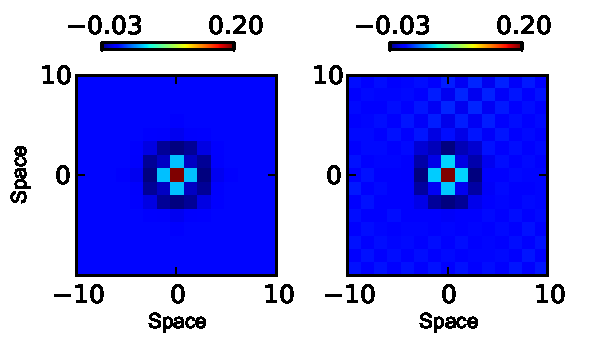
\includegraphics[width=0.5\textwidth]{./Graph/KernelEstimation2d.pdf}
 % \caption{Estimation of isotropic mixing kernel (Mexican-hat shape); left panel is the true kernel; right panel is the estimated kernel.}
 % \label{fig:MexHatKernel2d}
 % \end{figure} 
 % \begin{figure}[!h] 
 %  \centering
 %  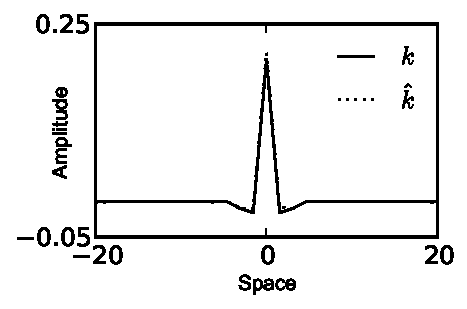
\includegraphics[width=0.5\textwidth]{./Graph/KernelSupportEstimation1d.pdf}
 %  \caption{Estimation of isotropic mixing kernel (Mexican-hat shape);  cross-sections of the true (at observation locations) and estimated kernels are shown by solid and dotted lines respectively .}
 %  \label{fig:MexHatKernel1d}
 %  \end{figure}   
% \begin{figure}[!h] 
%  \centering
%  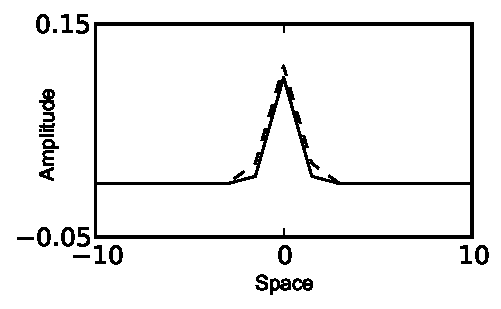
\includegraphics[width=0.5\textwidth]{./Graph/DisturbanceSupportEstimation1d.pdf}
%  \caption{Estimation of disturbance covariance function, $\sigma_d^2\gamma(\mathbf{r}-\mathbf{r'})$;  cross-sections of the true and estimated  kernels  are shown by solid and dashed lines respectively.}
%  \label{fig:EstimatedSupport1d}
%  \end{figure}     
\subsection{Example II: anisotropic mixing kernel}
For this experiment the homogeneous kernel parameters are set as $n_\theta=3$, $\boldsymbol\mu_0=-\boldsymbol\mu_2=[-0.5~-0.5]$ and $\boldsymbol\mu_1=[0~0]$. The widths  of the kernel components are equal and chosen to be $\sigma_i^2=5.76$ with $\theta_0=-0.07$, $\theta_1=0.07$ and $\theta_2=0.02$ resulting in anisotropic kernel shown in \figurename{\ref{fig:anisoKernel2d}} where the estimated kernel is also depicted. Cross-sections of plots in \figurename{\ref{fig:anisoKernel2d}} are shown in \figurename{\ref{fig:anisoKernel1d}}.
\begin{figure}[!h] 
 \centering
 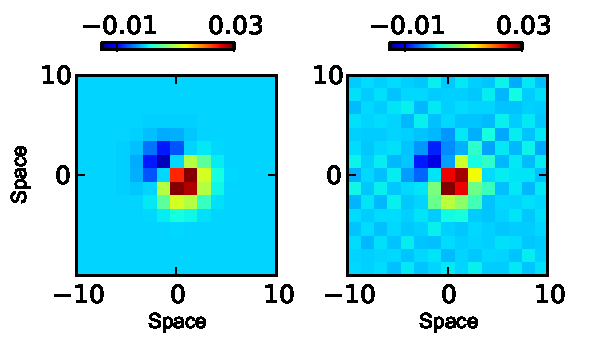
\includegraphics[width=0.5\textwidth]{./Graph/anisoKernelEstimation2d.pdf}
 \caption{Estimation of anisotropic mixing kernel; left panel is the true kernel; right panel is the estimated kernel.}
 \label{fig:anisoKernel2d}
 \end{figure}
% \begin{figure}[!h] 
%  \centering
%  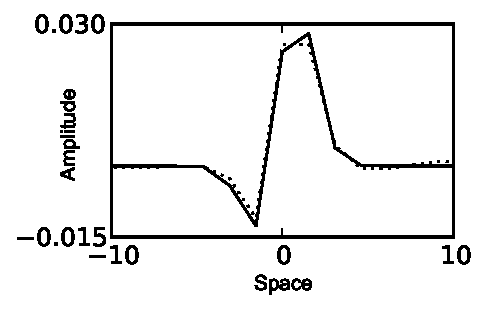
\includegraphics[width=0.5\textwidth]{./Graph/anisoKernelSupportEstimation1d.pdf}
%  \caption{Estimation of anisotropic mixing kernel;  cross-sections of the true (at observation locations) and estimated kernels are shown by solid and dotted lines respectively .}
%  \label{fig:anisoKernel1d}    
%  \end{figure}    

\begin{figure*}[ht]
	\centering
		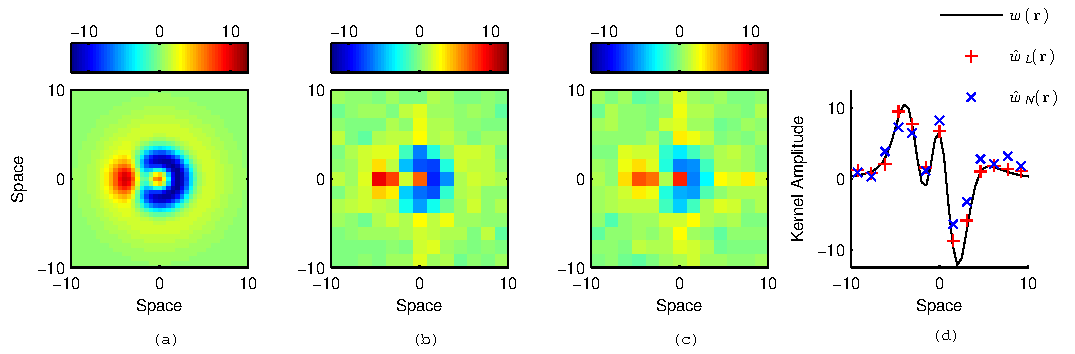
\includegraphics[scale=1]{./Graph/AnisoKernelIEEE.pdf}
	\caption{caption}
	\label{fig:label}
\end{figure*}

 \subsection{Example III: anisotropic mixing kernel}
For this experiment the homogeneous kernel parameters are set as $n_\theta=2$, $\boldsymbol\mu_0=-\boldsymbol\mu_2=[-0.5~-0.5]$. The widths  of the kernel components are equal and chosen to be $\sigma_i^2=5.76$ with $\theta_0=0.2$ and $\theta_1=-0.2$, resulting in anisotropic kernel shown in \figurename{\ref{fig:1anisoKernel2d}} where the estimated kernel is also depicted. Cross-sections of plots in \figurename{\ref{fig:1anisoKernel2d}} are shown in \figurename{\ref{fig:1anisoKernel1d}}.
\begin{figure}[!h] 
 \centering
 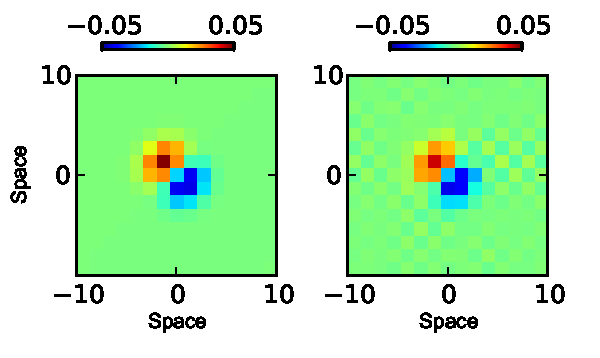
\includegraphics[width=0.5\textwidth]{./Graph/1anisoKernelEstimation2d.pdf}
 \caption{Estimation of anisotropic mixing kernel; left panel is the true kernel; right panel is the estimated kernel.}
 \label{fig:1anisoKernel2d}
 \end{figure}
% \begin{figure}[!h] 
%  \centering
%  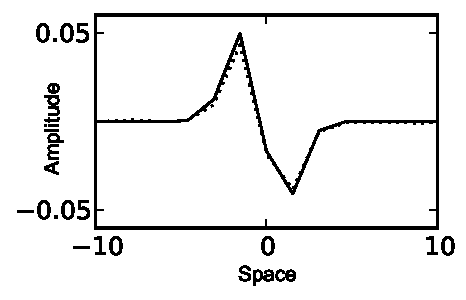
\includegraphics[width=0.5\textwidth]{./Graph/1anisoKernelSupportEstimation1d.pdf}
%  \caption{Estimation of anisotropic mixing kernel;  cross-sections of the true (at observation locations) and estimated kernels are shown by solid and dotted lines respectively .}
%  \label{fig:1anisoKernel1d}    
%  \end{figure}  
\section{Conclusion}
An efficient and novel approach to modeling spatio-temporal systems has been presented. This model is able to identify spatial mixing kernel, disturbance and noise characteristics from observed field. This ability greatly facilitates the identification of the class of system which the IDE can represent.


For more accurate estimation of the spatial kernel and also the inference of the underlying field the EM framework can be combined with the proposed method in this work. The estimated support of the kernel can be  used as a guide to constrain the placement of basis functions and the corresponding coefficients can be further corrected using the EM algorithm for more accurate representation of the mixing kernel structure. In fact, the correlation analysis can be considered a prerequisite for the EM algorithm described in \cite{Dewar2009}, where the approximated supports can be used to estimate the gain of the kernel and the field disturbance variance.                                             
                                                                                                                                                                              

An alternative to estimating the support of the kernel in a traditional state-space scheme is to place a regular grid of spatial mixing kernel basis functions over the entire spatial domain of the field. However, the estimate of the spatial extent of the mixing kernel greatly improves the speed of the estimation algorithm as the number of basis functions can be significantly reduced. This also improves the uncertainty in the estimated coefficients, as a lower number of unknown parameters needs to be estimated. 

The approximated support of the disturbance covariance function also facilitates the application of the EM algorithm for estimating the temporal variance in the disturbance signal. This way the disturbance covariance matrix can be decomposed into two parts: an unknown scalar and a constant matrix depending only on the inferred spatial support. Therefore, the estimation problem of the disturbance covariance matrix breaks down to the estimation of a single scalar parameter, improving the accuracy and the convergence property of the algorithm.

In the case where the spatial process is observed at irregular locations, spatial interpolation maybe possible to apply in order to obtain a regular grid of observations to perform the proposed estimation framework.




% if have a single appendix:
% \appendix[Convolution and Correlation]
% or
 \appendices  % for no appendix heading
% do not use \section anymore after \appendix, only \section*
% is possibly needed
% use appendices with more than one appendix
% then use \section to start each appendix
% you must declare a \section before using any
% \subsection or using \label (\appendices by itself
% starts a section numbered zero.)
%  ###########################################
 \section{Convolution and Correlation}\label{ap:CorrelationAnalysis}
In this appendix the properties of the cross-correlation and the convolution used in Section~\ref{sec:EstimationMethod}   are derived. To show 
\begin{equation}\label{eq:app-ConvXcorRelation1}
 \left(a \ast b \right)\left(\boldsymbol\tau\right)  \star c\left(\boldsymbol\tau\right)  = a\left(-\boldsymbol\tau\right)\ast\left(b \star c\right)\left(\boldsymbol\tau\right)
\end{equation}
and
\begin{equation}\label{eq:app-ConvXcorRelation2}
(a \ast b)(\boldsymbol \tau) \star (a \ast b)(\boldsymbol\tau)=(a \star a)(\boldsymbol\tau)\ast(b \star b)(\boldsymbol\tau),
\end{equation}
first note that cross-correlation function is related to the convolution by \cite{Yarlagadda2009}
\begin{equation}\label{eq:app-ConvXcorRelation}
 \left(a \star b\right)\left(\boldsymbol\tau\right)= a\left(-\boldsymbol\tau\right)\ast b\left(\boldsymbol\tau\right).
\end{equation}
Therefore, \eqref{eq:app-ConvXcorRelation1} can be written as
\begin{align}
 \left(a \ast b\right)\left(\boldsymbol\tau\right) \star c\left(\boldsymbol\tau\right)&= \left(a \ast b\right)\left(-\boldsymbol\tau \right)\ast c\left(\boldsymbol\tau\right) \nonumber \\
&=a\left(-\boldsymbol\tau\right)\ast \left(b\left(-\boldsymbol\tau\right) \ast c\left(\boldsymbol\tau\right)\right)\nonumber \\
&=a\left(-\boldsymbol\tau\right)\ast\left(b\star c\right)\left(\boldsymbol\tau\right).
\end{align}
Similarly, \eqref{eq:app-ConvXcorRelation2} can be written as
\begin{align}
 (a \ast b)(\boldsymbol \tau) \star (a \ast b)(\boldsymbol\tau)&=(a \ast b)(-\boldsymbol\tau) \ast (a \ast b)(\boldsymbol\tau) \nonumber \\
&=a(-\boldsymbol\tau)\ast a(\boldsymbol\tau) \ast b(-\boldsymbol\tau)\ast b(\boldsymbol\tau) \nonumber \\
&=(a \star a)(\boldsymbol\tau)\ast(b \star b)(\boldsymbol\tau).
\end{align}     
 \section{Linear IDE}\label{ap:linearIDE}  
Consider the following homogeneous linear IDE
\begin{equation}\label{app:DiscreteTimeModel}
	z_{t+1}\left(\mathbf{r}\right) = 
	\xi z_t\left(\mathbf{r}\right) + 
	T_s \int_\Omega { 
	    k\left(\mathbf{r}-\mathbf{r'}\right)z_t\left(\mathbf{r}'\right)
	\, \mathrm{d}\mathbf{r}'} 
	+ e_t\left(\mathbf{r}\right), 
\end{equation}              
then the results for the spatial mixing kernel and the covariance functions are simplified to
\begin{equation}\label{app:EM-KernelSolution}
	k(\boldsymbol\tau) = \frac{1}{T_s }\mathcal{F}^{-1}\overline{\left\{\frac{\mathcal{F}\{\mathbf{E}[R_{y_{t+1}y_t}(\boldsymbol{\tau})]\}}{\mathcal{F}\{(\mathbf{E}\left[R_{y_ty_t}(\boldsymbol\tau)\right]\} - \sigma_{\varepsilon}^2 }-\xi\right\}}.
\end{equation}  
and
\begin{align}\label{app:EM-MMGFourier2}
	&\gamma(\boldsymbol\tau) =\mathcal{F}^{-1}\left\lbrace \frac{1}{\tilde{m}(\boldsymbol\tau)}\Bigg[\left[\mathcal{F}\{\mathbf{E}[R_{y_{t+1}y_{t+1}}(\boldsymbol{\tau})]\}-\sigma_{\varepsilon}^2\right] \nonumber \right.\\
 &\left. \left.- \left[\frac{\mathcal{F}\{\mathbf{E}[R_{y_{t+1}y_t}(\boldsymbol{\tau})]\}\mathcal{F}\left\{\mathbf{E}\left[R_{y_ty_{t+1}}(\boldsymbol\tau)\right] \right\}}{\mathcal{F}\{(\mathbf{E}\left[R_{y_ty_t}(\boldsymbol\tau)\right]\} - \sigma_{\varepsilon}^2}\right]\right]\right\rbrace.
\end{align}                                                                                                                       
This is in fact a spacial case for the general solutions given by \eqref{eq:Fourier_TF_of_Kernel} and \eqref{eq:EM-MMGFourier2} with $\varsigma=4$ and $z_0=0.5$. This can be further simplified by setting the decay parameter, $\xi=0$ and sampling time, $T_s=1$. In this case the solution for the kernel is given by
\begin{equation}\label{app:EM-KernelSolution1}
	k(\boldsymbol\tau) =\mathcal{F}^{-1}\overline{\left\{\frac{\mathcal{F}\{\mathbf{E}[R_{y_{t+1}y_t}(\boldsymbol{\tau})]\}}{\mathcal{F}\{(\mathbf{E}\left[R_{y_ty_t}(\boldsymbol\tau)\right]\} - \sigma_{\varepsilon}^2 }\right\}}.
\end{equation}                      
while the disturbance covariance function solution remains unchanged, showing that the result is independent of the decay term. In this case the exact shape of the covariance function only depends on the observation noise variance and the observation kernel.
%\appendices
%\section{Proof of the First Zonklar Equation}
%Appendix one text goes here.

% you can choose not to have a title for an appendix
% if you want by leaving the argument blank
%\section{}
%Appendix two text goes here.


% use section* for acknowledgement
%\section*{Acknowledgment}

% Can use something like this to put references on a page
% by themselves when using endfloat and the captionsoff option.
\ifCLASSOPTIONcaptionsoff
  \newpage
\fi



% trigger a \newpage just before the given reference
% number - used to balance the columns on the last page
% adjust value as needed - may need to be readjusted if
% the document is modified later
%\IEEEtriggeratref{8}
% The "triggered" command can be changed if desired:
%\IEEEtriggercmd{\enlargethispage{-5in}}

% references section

% can use a bibliography generated by BibTeX as a .bbl file
% BibTeX documentation can be easily obtained at:
% http://www.ctan.org/tex-archive/biblio/bibtex/contrib/doc/
% The IEEEtran BibTeX style support page is at:
% http://www.michaelshell.org/tex/ieeetran/bibtex/
 % \newpage
\bibliographystyle{IEEEtran}
% argument is your BibTeX string definitions and bibliography database(s)
\bibliography{IEEEabrv,IEEECorr}  
% <OR> manually copy in the resultant .bbl file
% set second argument of \begin to the number of references
% (used to reserve space for the reference number labels box)

% \begin{thebibliography}{1}
% 
% \bibitem{IEEEhowto:kopka}
% H.~Kopka and P.~W. Daly, \emph{A Guide to \LaTeX}, 3rd~ed.\hskip 1em plus
%   0.5em minus 0.4em\relax Harlow, England: Addison-Wesley, 1999.
% 
% \end{thebibliography}

% biography section
% 
% If you have an EPS/PDF photo (graphicx package needed) extra braces are
% needed around the contents of the optional argument to biography to prevent
% the LaTeX parser from getting confused when it sees the complicated
% \includegraphics command within an optional argument. (You could create
% your own custom macro containing the \includegraphics command to make things
% simpler here.)
%\begin{biography}[{\includegraphics[width=1in,height=1.25in,clip,keepaspectratio]{mshell}}]{Michael Shell}
% or if you just want to reserve a space for a photo:
% \begin{IEEEbiography}{Parham Aram}
% 
%  
% \end{IEEEbiography}
% 
% \begin{IEEEbiography}{Visakan Kadirkamanathan}
% % Biography text here.
% (M’90) received the
% B.A. and Ph.D. degrees in electrical and information
% engineering from the University of Cambridge, U.K.
% He held Research Associate positions at the University
% of Surrey, U.K., and the University of Cambridge,
% U.K., before joining the Department of Automatic
% Control and Systems Engineering, The University
% of Sheffield, U.K., as a Lecturer in 1993, where
% he is currently a Professor of Signal and Information
% Processing and is affiliated to the Centre for Signal
% Processing and Complex Systems. His research interests
% include nonlinear signal processing, system identification, intelligent control
% and fault diagnosis with applications in systems biology, aerospace systems,
% and wireless communication. He has coauthored a book on intelligent control
% and has published more than 120 papers in refereed journals and proceedings of
% international conferences.
% Prof. Kadirkamanathan is the Co-Editor of the International Journal of Systems
% Science and has served as an Associate Editor for the IEEE TRANSACTIONS
% ON NEURAL NETWORKS and the IEEE TRANSACTIONS ON SYSTEMS, MAN, AND
% CYBERNETICS, PART B.
%  \end{IEEEbiography}
% \begin{IEEEbiography}{Michael Dewar}
%  received the M.Eng. degree in
% control systems engineering and the Ph.D. degree
% in systems engineering both from The University of
% Sheffield, U.K., in 2002 and 2007, respectively.
%  He is currently working as
% a Research Associate in the Institute for Adaptive
% and Neural Computation, School of Informatics,
% The University of Edinburgh, U.K. 
% \end{IEEEbiography}

% if you will not have a photo at all:
% \begin{IEEEbiographynophoto}{John Doe}
% Biography text here.
% \end{IEEEbiographynophoto}

% insert where needed to balance the two columns on the last page with
% biographies
%\newpage

% \begin{IEEEbiographynophoto}{Jane Doe}
% Biography text here.
% \end{IEEEbiographynophoto}

% You can push biographies down or up by placing
% a \vfill before or after them. The appropriate
% use of \vfill depends on what kind of text is
% on the last page and whether or not the columns
% are being equalized.

%\vfill

% Can be used to pull up biographies so that the bottom of the last one
% is flush with the other column.
%\enlargethispage{-5in}



% that's all folks
\end{document}


